%===План каждой из трёх подсекций===
%Эксперимент XXXX
%   число событий в секунду
%   число измеримых частиц в событии
%Детектор XXXX RICH
%   импульс измеримых электронов
%   дискриминация от каких частиц
%   в каком диапазоне импульсов
%   угловой аксептанс
%Корпус и радиатор
%   материал и толщина корпуса на входе и выходе
%   тип и состав радиатора
%   давление радиатора
%   активная длина радиатора
%Зеркала и опоры
%   материал
%   гранулярность
%   радиус кривизны
%   площадь
%   наличие дополнительных зеркал
%   краткая характеристика системы поддержки зеркал
%Фотодетекторы
%   тип фотодетектора
%   число каналов
%   размер "пикселя" или шага проволочек
%Электроника
%   считывающая электроника
%   наличие/отсутствие внешнего триггера


\section{Обзор существующих детекторов черенковских колец}\label{sec:secRiches}

Использование детекторов черенковских колец со сферическими фокусирующими зеркалами для идентификации частиц имеет долгую историю~\cite. Следуя за постоянно возрастающими требованиями со стороны экспериментов, а также используя новейшие технологические достижения в различных областях, все основные подсистемы детекторов RICH прошли впечатляющую эволюцию. К основным подсистемам можно отнести фокусирующие зеркала, системы фиксации и корректировки положения зеркал, системы газообеспечения, оболочку корпуса, фотодетекторы и системы считывания. Детектор CBM RICH, которому посвящена данная работа, опирается в той или иной степени на опыт нескольких экспериментов предыдущего поколения. В нижеследующей секции будут описаны несколько приборов, сравнение с которыми позволит понять уникальное место CBM RICH в ряду аналогичных установок.

% ==========================================================================================
% ==========================================================================================
% ==========================================================================================

\subsection{COMPASS RICH-1}\label{sec:CompassRich1}

% Википедия
% https://en.wikipedia.org/wiki/COMPASS_experiment

\subsubsection{Эксперимент COMPASS}

Экспериментальная установка NA58, также известная как COMPASS (``Common Muon and Proton Apparatus for Structure and Spectroscopy'') представляет собой систему из двух спектрометров длиной 60~метров за неподвижной мишенью на отводе пучка M2 ускорителя SPS в CERN. Эксперимент был предложен в 1996 году, в период с 1999 по 2001 года выполнялись работы по установке и в 2001 был выполнен первый (commissioning) запуск. Набор данных разбит на два этапа: COMPASS I (2002--2011) и COMPASS II (2012--2018). 

% http://link.springer.com/article/10.1140/epjst/e2008-00800-2

% Самое свежее (2014) - http://compassweb.ts.infn.it/rich1/paper/tessarotto_instr14.pdf

% Ссылки
% NIM A 02 (2003) 112–116
% doi:10.1016/S0168-9002(02)02165-4
% E. Albrecht et al.
% https://wwwcompass.cern.ch/compass/detector/rich/publications/NIMA502-112.pdf

% http://wwwcompass.cern.ch/compass/proposal/pdf/proposal.pdf

% https://pub.uni-bielefeld.de/download/2301233/2301236
% 8.2.2 The Mirror Wall

\subsubsection{Общие слова о COMPASS RICH и его физической задаче}

Детектор Черенковских колец \mbox{RICH-1} был спроектирован в 1996~г. и функционирует с 2002~г. \mbox{RICH-1} подвергается постоянной оптиимизации, а в 2006~было выполнено обновление. Ожидается второе обновление детектора в 2016~г. \todo оно было?

Основная задача детектора Черенковских колец --- разделение $\pi$, $p$ и $K$ в диапазоне импульсов от 3~до~55~ГэВ/с в условиях высокой интенсивности (что бы это значило\todo в статье 2014 г. написано, что beam rate 40 МГц, и частота триггеров 20 кГц) в полном аксептансе спектрометра, составляющем $\pm$250~мрад по горизонтали и $\pm$180~мрад по вертикали. Для минимизации отрицательного влияния на эффективность стоящих ниже по пучку электромагнитного и адронного калориметров детектор \mbox{RICH-1} должен иметь минимум количества материала в аксептансе. Также в процессе проектирования COMPASS \mbox{RICH-1} необходимо было развивать технологии для реализации возможности регистрировать и справляться с высоким для того времени потоком данных.
\todo \textbf{По большому счёту, задачи те же, что и у CBM}

http://localhost/Lib/1-s2.0-S0168900203027499-main.pdf

In the 2002 run data were taken with a muon beam of 160~\GeVoverC and an intensity of $2 \cdot 10^{8}$ muons per spill of 4.8~s and a machine cycle of 16.8~s

\subsubsection{Корпус и радиатор}

Габариты корпуса детектора COMPASS \mbox{RICH-1}, выполненного из алюминия, составляют 6.6$\times$5.3$\times$3.3~м$^3$. Внутри расположен газовый радиатор $C_{4}F_{10}$ длиной 3~м и объёмом около 83~м$^3$. Пороги по импульсу для Черенковского света: для $\pi$ --- 2.5~ГэВ/с, для $K$ --- 8.9~ГэВ/с и 17~ГэВ/с для $p$. В центре детектора проходит цилиндрический ионопровод диаметром 100~мм, наполненный гелием.
% The original beam pipe, made of 150 mm thick stainless steel, has been replaced in 2012 by a lighter pipe, made of 4 layers of metalized BoPET (25mm BoPET + 0.2mm Al): the contribution to the total material budget by the new pipe for beam particles is 0.08\% X0 (plus 0.06\% due to helium).
Газовая система закрытого типа поддерживает радиатор под избыточным давление $100\pm10$~Па.
Передняя и задняя стенки корпуса выполнены из тонких алюминиевых плёнок спрессованных с жёсткой пеной. \todo
%http://localhost/Lib/NIMA502-112.pdf
%The front and rear vessel windows are sandwiches of two thin Al foils and a layer of rigid foam.

\subsubsection{Зеркала и опоры}

Система фокусировки состоит из двух сферических зеркал радиусом 6.6~м, составленных из 116~сегментов шести- и пятиугольной формы, общей площадью более 21~м$^2$. Для фокусировки на фоточувствительные камеры, расположенные за пределами геометрического аксептанса, центры сфер зеркал смещены по вертикали от пучка на 1.6~м, а образовавшийся в результате этого зазор между двумя зеркалами приводит к потере 4\% площади отражающей поверхности. Зеркала были произведены компанией IMMA, Ltd., Kinskeho 703, Turnov, Czech Republic.
Коллаборацией COMPASS был разработан метод контроля индивидуальных отклонений сегментов зеркал ``на лету'' (онлайн), называемый CLAM (``a continuous line alignment and monitoring method'').

Отражающая поверхность состоит алюминиевого слоя толщиной 80~нм, нанесённого на боросиликатное стекло толщиной 7~мм, и покрытого защитным слоем из $MgF_{2}$ толщиной 30~нм.
%The reflecting surface consists of an 80~nm thick $Al$ layer deposited on a 7~mm thick borosilicate glass substrate and covered by a 30~nm tick $MgF_{2}$ protective layer.

The mechanical structure supporting the mirror wall has a net-like configuration with spherical design made from aluminum. Each mirror is coupled to a fine thread screw which allows it to rotate around two orthogonal axes.

\todo \textbf{картинка - схема, оч похоже на CBM}

\subsubsection{Фотодетекторы}

Исходя из необходимости иметь суммарную площадь фоточувствительных камер 5.3~м$^2$, изначально для реализации были выбраны многопроволочные пропорциональные камеры (MWPC) с сегментированным фотокатодом из CsI. \mbox{RICH-1} оборудован восемью идентичными камерами, каждая площадью 576$\times$1152~мм$^2$. Фотокатоды выполнены из двух двухсторонних печатных плат размером 576$\times$576~мм$^2$. Окна из silica-quartz состоят из двух одинаковых quartz-plates размером 600$\times$600$\times$5~мм$^3$. Сегментированный фотокатод обеспечивает размер пикселя 8$\times$8~мм$^2$ и в общей сложности 82944 канала.

% Ещё подробности тут: http://localhost/Lib/Long_term_experience_and_performance_of_COMPASS_RI.pdf

В 2006~г. с целью повышения эффективности детектора было выполнено комплексное обновление центральной области фоточувствительной камеры, составляющей 25\% от всей площади. MWPC были заменены на МА~ФЭУ с индивидуальными линзами и соответствующей считывающей электроникой. В общей сложности было установлено 4 панели по 144~МА~ФЭУ Hamamatsu R7600-03-M16, имеющими 16~каналов и входное стекло, прозрачное в ультрафиолетовой области, и специальный делитель напряжения.

% For the physics runs starting in 2016 COMPASS RICH-1 will be equipped with new MPGD-based photon detectors, which have been developed by a dedicated R&D program.

\subsubsection{Электроника}

Сигнал с МА~ФЭУ считывается платами передней электроники, основанными на ASIC ``CMAD'', реализующем 8-канальный предусилитель-дискриминатор, разработанный на основе ``MAD4'' специально для COMPASS \mbox{RICH-1}. CMAD позволяет работать на частоте до 5~МГц на канал.

%The signals from the MAPMTs are read by a fast digital electronics system [36, 37] based on the 8 channels CMAD [38] preamplifier-discriminator, developed for COMPASS RICH-1 as an upgraded version in CMOS technology of the MAD4 [39] front-end chip. The CMAD has a small noise level (1 fC), the possibility to set individual channel thresholds, a good time resolution and high rate capability: it provides full efficiency up to an input rate of 5 MHz per channel. The design of the front-end boards and the optimization of the thresholds setting allows to completely suppress the MAPMTs cross talk signals while keeping the single photoelectron detection efficiency at a 95\% level.

\todo \textbf{перефразировать}
Хорошее временное разрешение МА~ФЭУ не портится за счёт использования цифровых карт DREISAM, в которых реализован ВЦП F1, имеющий временное разрешение 110~пс и может работать с чатотой до 10~МГц на канал и частоте триггера до 100~кГц.

%The good MAPMT time resolution is fully exploited with the help of digital cards, called DREISAM, housing the dead-time free F1 TDC [40] , which has a time resolution of 110 ps and can stably operate up to 10 MHz per channel input rate and 100 kHz trigger rate.

Считывающая электроника COMPASS \mbox{RICH-1} монтируется на детектор, образуя очень компактную установку, которая экранирована от внешнего электромагнитного поля медными пластинами, выполняющими также и роль радиаторов, охлаждаемых водой циркуирующей по медным трубкам.

%All the electronics components of the RICH-1 readout system are directly mounted on the detector and form a very compact setup. Each PCB is coupled to a copper plate providing both efficient electromagnetic shielding and good cooling power: thermalized water circulates in underpressure condition in thin copper pipes brazed onto the copper plates [36]. The stability and uniformity of the water cooling system has been achieved after several improvements of the distribution system and of the operation and maintenance protocols.

Оцифрованные данные с плат передней электроники передаются по оптике платам считывания CATCH, которые группируют данные и передают дальше также по оптике через S-LINK в систему сбора данных эксперимента.

%Data from the front-end cards are transferred via optical links to a set of CATCH readout-driver modules which concentrate the data and send them via S-LINK transmitter and optical fibre to the COMPASS DAQ system.

%Expected occupancy level is $\approx$5\% at a maximum trigger rate of $10^5 s^{-1}$, resulting in a maximum data flow of 2.5 GB/s. COMPASS-Gassiplex chips are used as front-end-chips. These are modified versions of the chips developed for RD26, now equipped with preamplifier, shaper and an analog-multiplexer. The intrinsic dead time is 400 nsec per event, with a peaking time of 1 usec. The value for noise is as low as 1100 electrons equivalent at a gas amplification of $\approx$6.5 mV / (fC).

%The core piece of the readout system is the total amount of 192 front-end-cards, the 60 cm long BORA boards [67], hosting the front-end chips and a first trigger level. There are 24 BORA-boards per photon chamber handling 432 analog channels. Each single BORA-board is equipped with front-end-chips, ADCs (analog digital converter), FIFOs (first in first out buffer), FPGAs (field programmable gate array) of the type VIRTEX XCV100 [68] for logic sequencers, threshold-subtraction and zero-suppression, 32-bit DSPs [69] for event packaging, on-board controls and optical links. The event processing time is 10usec. The control system for those BORA-boards is a parallel network of DSPs (digital signal processing), operated via a dedicated PC-PCI-interface: the DOLINA-boards with 8 on-board DSPs each. To avoid grounding interference between the PC and the detector all BORA-boards are optoisolated from DOLINA with the help of specific optoisolating boards. Figure 8.11 sketches the architecture of the readout system. The photon detectors reach an absolute gain of 10 4 at nominal voltage of 2000 V with photon detection efficiencies of about 75\% as presented in Figure 8.12.

\textbf{Заключение такое, что в целом конструкция этого RICH очень схожа с конструкцией CBM RICH.}

% ==========================================================================================
% ==========================================================================================
% ==========================================================================================

\subsection{LHCb}\label{sec:LHCb}

% http://localhost/Lib/10.1.1.668.3561.pdf - An Overview of the Status of the LHCb RICH Detectors - 2008

%\todo \textbf{ПРОСТО ЦЕЛИКОМ ПЕРЕВЕСТИ СЕКЦИЮ 2.1 ОТСЮДА:}
%http://localhost/Lib/art_10.1140_epjc_s10052-013-2431-9.pdf
% Performance of the LHCb RICH detector at the LHC - 2013

\subsubsection{Эксперимент LHCb}

LHCb --- один из четырёх крупных экспериментов на Большом Адронном Коллайдере (LHC). LHCb посвящён изучению нарушения CP-инвариантности и редких распадов тяжёлых ароматов. Он представляет собой прямой спектрометр, спроектированный принимать летящие прямо b- и c-адроны, рождённые в $p-p$ столкновениях. Схема установки LHCb показана на \figref{fig:LHCb}.

%LHCb is one of the four major experiments at the LHC, and is dedicated to the study of CP violation and the rare decay of heavy flavours. It is a forward spectrometer designed to accept forward-going b- and c-hadrons produced in proton-proton collisions. The layout of the spectrometer is shown in \figref{fig:LHCb}.

\textbf{Википедия:}
Основными задачами эксперимента LHCb являются: изучение редких эффектов CP-нарушения в распадах прелестных адронов, измерение углов треугольника унитарности, прецизионная проверка предсказаний Стандартной Модели (СМ) в редких радиационных, полулептонных и лептонных распадах B-мезонов, изучение редких распадов очарованных частиц и экзотических распадов $\tau$-лептонов.

\begin{figure}[H]
\centering
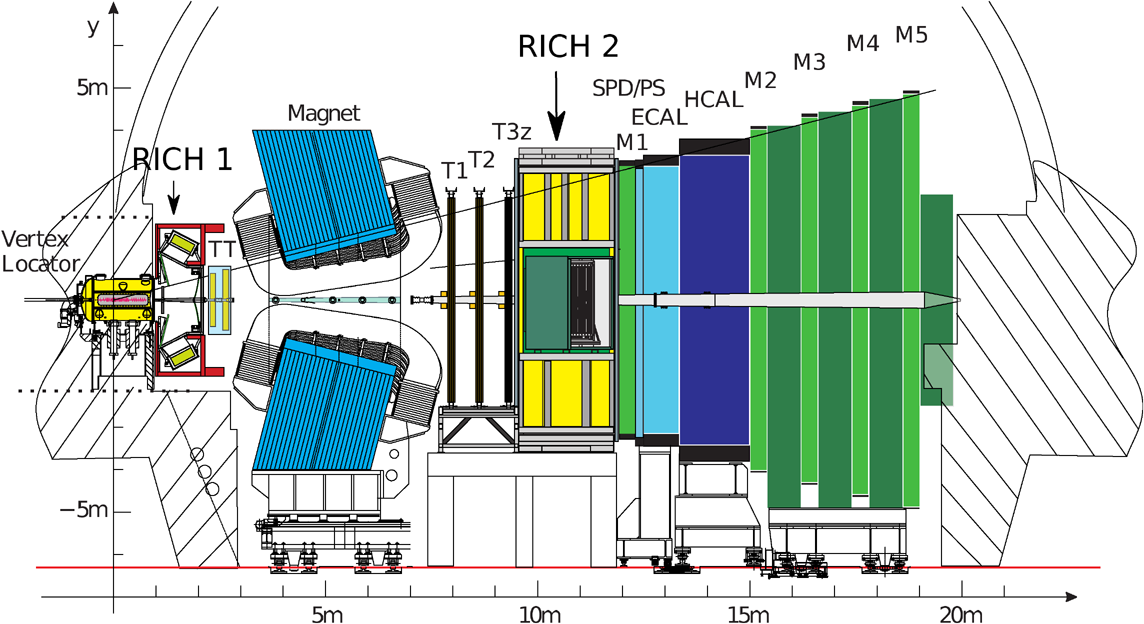
\includegraphics[width=1.0\textwidth]{pictures/LHCb.png}
\caption{Схема установки LHCb.}
\label{fig:LHCb}
\end{figure}

\subsubsection{Общие слова о LHCb RICH и его физической задаче}

LHCb RICH обеспечивает идентификацию частиц в диапазоне импульсов от 2 до 100~\GeVoverC. Два детектора черенковских колец полностью охватывают необходимый угловой аксептанс 15--300 мрад with respect to the beam axis.

RICH1 покрывает нижний и средний диапазон импульсов от 2 до 40~\GeVoverC во всём угловом аксептансе 25--300 мрад. Ограничение снизу возникает от размера ионопровода (выше по пучку \todo). RICH2 покрывает диапазон высоких импульсов от 15 до 100~\GeVoverC в области 15--120 мрад.

RICH1 covers the low and intermediate momentum region 2–40~\GeVoverC over the full spectrometer angular acceptance of 25–300 mrad. The acceptance is limited at low angle by the size of the beampipe upstream of the magnet. RICH2 covers the high-momentum region 15–100~\GeVoverC, over the angular range 15–120 mrad.

\subsubsection{Корпус и радиатор}

\mbox{RICH-1} расположен максимально близко к точке взаимодействия, насколько это возможно. С целью минимизации количества материала у \mbox{RICH-1} нет отдельного входного окна --- в качестве передней стенки контейнера для газового радиатора используется выходная стенка вакуумной камеры детектора VELO. Выходное окно \mbox{RICH-1} изготовлено из лёгкого материала, представляюшего собой ``сэндвич'' из углепластика и пены.

%\mbox{RICH-1} is placed as close as possible to the interaction region. To minimize the material budget there is no separate entrance window, and the \mbox{RICH-1} gas enclosure is sealed directly to the exit window of the VELO vacuum tank. The downstream exit window is constructed from a low-mass carbon-fibre/foam sandwich.

\mbox{RICH-2} располагается за магнитом, т.к. треки с высоким импульсом, которые он измеряет, меньше подвержены воздействию магнитного поля. Благодаря этому \mbox{RICH-2} может быть помещён за трекинговыми детекторами для уменьшения количества материала, что оказывает положительное влияние на регистрацию треков заряженных частиц. Так же, как и в случае \mbox{RICH-1}, входное и выходное окна \mbox{RICH-2} выполнены из легких сэндвич-панелей из пористого материала, покрытых углепластиком и алюминием соответственно.

%\mbox{RICH-2} is placed downstream of the magnet, since the high momentum tracks it measures are less affected by the magnetic field. In this way it can be placed after the downstream tracking system in order to reduce material for the measurement of the charged tracks. The entrance and exit windows are again a foam sandwich construction and skinned with carbon-fibre and aluminium, respectively.

По причине низкой дисперсии в качестве Черенковских радиаторов используются фтор-углеродные газы --- $C_{4}F_{10}$ в RICH1 и $CF_{4}$ в RICH2 --- при комнатной температуре и нормальном давлении. Коэффициенты преломления соответственно равны 1.0014 и 1.0005 при $\SI{0}{\degreeCelsius}$, 101.325~кПа и 400~нм. Около 5\% $CO_{2}$ было добавлено в $CF_{4}$ для погашения сцинтилляции в газе.

%Fluorocarbon gases at room temperature and pressure are used as Cherenkov radiators; C4F10 in RICH 1 and CF4 in RICH 2 were chosen for their low dispersion. The refractive index is respectively 1.0014 and 1.0005 at 0 C, 101.325 kPa and 400 nm. About 5\% CO2 has been added to the CF4 in order to quench scintillation in this gas.

Порог по импульсу для черенковского света в $C_{4}F_{10}$ составляет 9.3~\GeVoverC. Частицы с меньшим импульсом идентифицируются как каоны, а не пионы в режиме запрета \todo, то есть \todo.
Чтобы поддерживать положительную идентификацию при низких импульсах и для того чтобы разделять каоны и протоны, в RICH1 был включён второй радиатор: стенка толщиной 50~мм, составленная из 16~плиток silica аэрогеля, была помещена при входе в RICH1. Коэффициент преломления равен 1.03, а light scattering length \todo составляет прилизительно 50~мм при длине волны 400~нм в чистом $N_2$. Аэрогель помещён в $C_{4}F_{10}$ \todo и тонкий стеклянный фильтр ограничивает дисперсию \todo

%The momentum threshold for kaons to produce Cherenkov light in C4F10 is 9.3 GeV/c. Particles below this momentum would only be identified as kaons rather than pions in veto mode, i.e. by the lack of Cherenkov light associated to the particle. To maintain positive identification at low momentum and in order to separate kaons from protons, a second radiator is included in RICH 1: a 50 mm thick wall made of 16 tiles of silica aerogel [10] at the entrance to RICH 1. The refractive index is n=1.03 and the light scattering length is around 50 mm at 400 nm in pure N2. The aerogel is placed in the C4F10 gas volume and a thin glass filter is used on the downstream face to limit the chromatic dispersion.

\subsubsection{Зеркала и опоры}

Оба детектора имеют схожую оптическую систему, состоящую из наклонённых сферических зеркал в паре с плоскими зеркалами. Наличие двух зеркал позволяет значительно сократить габариты детектора вдоль направления пучка. Каждая оптическая система разделена на две половины: \mbox{RICH-1} --- симметрично относительно горизонтальной оси, \mbox{RICH-2} --- симметрично относительно вертикальной оси. Разделение фокусирующей и детектирующий подсистем \mbox{RICH-1} на симметричные половины было выполнено из-за необходимости наличия магнитного экрана вокруг фотодетекторов для защиты от магнитного поля от расположенного в непосредственной близости дипольного магнита.
Сферические зеркала \mbox{RICH-1} (4 сегмента) собраны из четырёх квадрантов на углепластиковой опоре, в то время как зеркала \mbox{RICH-2} (56 сегментов) и все плоские зеркала (16 и 40 сегментов у \mbox{RICH-1} и \mbox{RICH-2} соответсвенно) собраны из более мелких элементов \todo

The \mbox{RICH-1} detector utilizes innovative carbon-fibre mirror. \todo

%https://lhcb-public.web.cern.ch/lhcb-public/en/Detector/RICH2-en.html
%Particles produced in the collisions in LHCb will travel through the mirrors of \mbox{RICH-1} prior to reaching measurement components further downstream. To reduce the amount of scattering, \mbox{RICH-1} uses special lightweight spherical mirrors constructed from a carbon-fibre reinforced polymer (CFRP), rather than glass. There are four of these mirrors, each made from two CFRP sheets moulded into a spherical surface with a radius of 2700 mm and separated by a reinforcing matrix of CFRP cylinders.

%http://localhost/Lib/1-s2.0-S0168900214004975-main.pdf
%The result of the optics redesign was that the radius of curvature of the spherical mirror was increased from 2710~mm to 3800~mm and it was moved downstream by 86~mm.

%http://localhost/Lib/0303012.pdf
%To be able to place the focal surface outside the particle flux ($\pm$160 mrad vertically), the mirror is split horizontally and both halves are tilted by $\SI{9}{\degree}$ away from the beam-line.

\todo

%Both RICH detectors have a similar optical system, with a tilted spherical focusing primary mirror, and a secondary flat mirror to limit the length of the detectors along the beam direction. Each optical system is divided into two halves on either side of the beam pipe, with RICH 1 being divided vertically and RICH 2 horizontally. The vertical division of RICH 1 was necessitated by the requirements of magnetic shielding for the photon detectors, due to their close proximity to the magnet.
%The spherical mirrors of RICH 1 (4 segments) are constructed in four quadrants, with carbon-fibre structure, while those of RICH 2 (56 segments), and all flat mirrors (16 and 40 segments in RICH 1 and RICH 2 respectively), are tiled from smaller mirror elements, employing a thin glass substrate.


\subsubsection{Фотодетекторы}

Черенковские фотоны, рождённые заряженной частицей, проходящей вквозь радиаторы, фокусируются в (изображения \todo) кольца на плоскости фотодетекторов, расположенные за пределами аксептанса спектрометра. Инновационные гибридные фотодетекторы (HPD) были разработаны в сотрудничестве с индустрией специально для применения в LHCb RICH. HPD представляют собой вакуумную трубку, имеющую активный диаметр 75~мм, с кварцевым окном и многощелочной фотокатод. Фотоэлектроны фокусируются на массив кремниевых пикселей посредством ускоряющего напряжения -16~кВ. Пиксели организованы в массив $32 \times 32$, давая 1024 пикселя на трубку. Размер пикселя составляет $2.5 \times 2.5~mm^{2}$ на уровне фотокатода \todo В общей сложности 484~HPD плотно упакованы, формируя 4~плоскости фотодетекторов. Каждый из двух RICH детекторов использует две плоскости, 196~HPD в RICH1, 288 --- в RICH2.
Плоскости фотодетекторов отделены от радиатора кварцевым окном, что позволяет содержать HPD в $CO_{2}$. Чипы передней электроники смонтированы непосредственно в вакуумном пространстве внутри HPD \todo.

%The Cherenkov photons emitted by charged particles passing through the RICH radiators are focused into ring images on the photon detector planes, situated outside of the spectrometer acceptance. A novel hybrid photon detector (HPD) was developed in collaboration with industry specifically for application in the LHCb RICH system [11]. The HPDs employ vacuum tubes with a 75~mm active diameter, with a quartz window and multialkali photocathode. The photoelectrons are focused onto a silicon pixel array, using an accelerating voltage of -16~kV. The pixel array is arranged in 32~columns and 32~rows, giving a total of 1024 pixels per tube. The pixel size is $2.5 \times 2.5~mm^{2}$ at the level of the photocathode. A total of 484 HPDs are close-packed to cover the four photodetector planes. Two planes are employed in each RICH, with 196~tubes used in RICH1 and 288 in RICH2.
The photodetector planes are separated from the radiator gas volumes by quartz windows, and the photodetector volumes are maintained in an atmosphere of CO2 . The front-end electronics chip is encapsulated within the HPD vacuum tube, and bump-bonded to the silicon pixel sensor, which results in extremely low noise (typically 150 e- RMS per pixel for a signal of 5000 e- [12,13]). The tubes also feature high detection efficiency, with an active area fraction of about 82\%. The quantum efficiency is about 30\% at 270 nm.

\subsubsection{Электроника}

% ==========================================================================================
% ==========================================================================================
% ==========================================================================================

\subsection{HERA-b RICH}\label{sec:HerabRich}

% http://localhost/Lib/rich-instr99-nim453.pdf
% 0303012.pdf - The HERA-B Ring Imaging Cerenkov Counter

\subsubsection{Эксперимент HERA-b}

% Википедия
% https://en.wikipedia.org/wiki/HERA-B
% http://images.slideplayer.com/28/9404350/slides/slide_5.jpg

HERA (нем. Hadron-Elektron-RingAnlage или англ. Hadron-Electron Ring Accelerator) --- первый и единственный на данный момент лептон-протонный коллайдер, функционировавший с 1992~г. по 2007~г. в DESY, Гамбург, Германия. HERA-b --- один из четырёх экспериментов на HERA --- представляет собой эксперимент с фиксированной мишенью для измерения редких распадов B-мезонов, рождающихся в столкновениях протонов с импульсом 920~\GeVoverC{} с фиксированной мишенью.
Схема экспериментальной установки представлена на \figref{fig:HERAbSetup}.

Отличительной особенностью этого эксперимента является то, что в роли мишени выступали 8 проволочек из различных материалов, помещаемых в гало протонного пучка. Предполагалось, что такой инновационный метод позволит избежать влияния на пучок, что позволит выполнять измерения при невероятно высоких частотах взаимодействия (5--10~МГц).
\todo

%HERA-B, a fixed target experiment (see Fig. 1) at the HERA storage ring at DESY, was designed [1] to measure rare processes in the decays of B mesons. The B mesons are produced in collisions of 920 GeV/c protons with a fixed target, which consists of 8 wires which can be individually inserted into the halo of the proton beam in order not to disturb experiments measuring ep collisions. 


\begin{figure}[H]
\centering
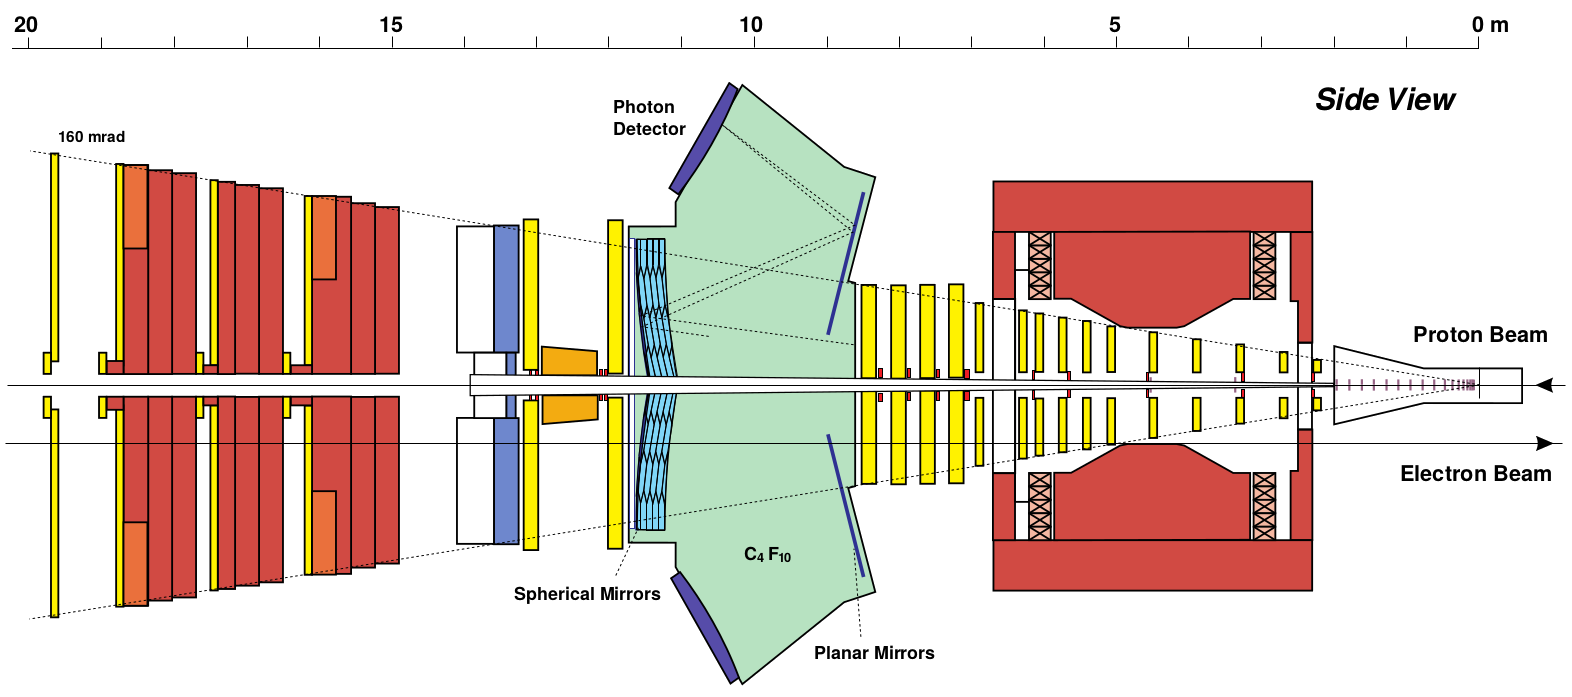
\includegraphics[width=1.0\textwidth]{pictures/HERA_b_setup.png}
\caption{Схема установки HERA-b.}
\label{fig:HERAbSetup}
\end{figure}

\subsubsection{Общие слова о HERA-b RICH и его физической задаче}

HERA-b RICH --- один из основных компонентов спектрометра HERA-b. Его основная задача --- идентификация заряженных адронов, в частности каонов, рождающихся в распадах B-мезонов. Идентификация заряженных каонов означает их отделение от пионов в диапазоне импульсов 3--5~\GeVoverC{} при частоте первичных взаимодействий до 40~МГц.

One of the essential components of the spectrometer is the Ring Imaging Cherenkov counter (RICH). The main purpose of the RICH counter is the identification of charged hadrons, in particular kaons from decays of B mesons. Identifying charged kaons essentially means separating them from pions in the momentum range between 3~\GeVoverC{} and about 50~\GeVoverC{} at an interaction rate of up to 40 MHz.

\subsubsection{Корпус и радиатор}

Схема детектора RICH эксперимента HERA-b показана на \figref{fig:HERAbRICH}. Он имеет газовый радиатор $C_{4}F_{10}$ объёмом 108~м$^3$ и массой 1100~кг. Длина радиатора 2.8~м, коэффициент преломления n=1.00137, порог импульса для рождения Черенковских фотонов для пионов и каонов составляет 2.7~\GeVoverC и 9.6~\GeVoverC соответственно. Для частиц с $\beta=1$ Черенковский угол равен 51.5~мрад (52.4~мрад), а разница между пионами и каонами составляет 0.9~мрад при 50~\GeVoverC. Радиатор поддерживается при избыточном давлении 2.5~мбар.

Корпус детектора изготовлен из нержавеющей стали, кроме передней и задней стенок из алюминия толщиной 1~мм. После фокусировки фотоны выходят из корпуса через стенку толщиной 2~мм из оргстекла прозрачного в ультрафиолетовой области. Передняя стенка HERA-b RICH расположена на расстоянии 8.5~м от мишени.

\subsubsection{Зеркала и опоры}

Система фокусировки состоит из двух пар зеркал, расположенных симметрично относительно горизонтальной плоскости, проходящей через ось пучка. Первое зеркало сферическое, второе --- плоское. Сферические зеркала (см. \figref{fig:HERAbRICHmirrors}) составлены из 80 полных или обрезанных шестиугольных сегментов, имеют радиус 11.4~м и толщину 7~мм. Они покрывают прямоугольную область 6$\times$4~м, общая площадь 24~м$^2$. Каждый сегмент крепится к раме трёмя моторизированными актуаторами с удалённым управлением. Для фокусировки за пределы геометрического аксептанса сферические зеркала наклонены на $\SI{9}{\degree}$ от пучка. Каждое из двух плоских зеркал состоит из 18 сегментов.

%http://localhost/Lib/0303012.pdf 3.2

The mirror, a 6 m by 4 m rectangular cutout from the sphere, consists of 80 full or partial hexagons made from 7 mm thick Pyrex glass, coated with 200 nm of aluminum and 30 nm of $MgF_{2}$.

\subsubsection{Фотодетекторы}

HERA-b RICH имеет две фоточувствительные камеры, расположенные соответственно над и под пучком. Одна фоточувствительная камера (см. \figref{fig:HERAbRICHcamera}) составлена из 7 супермодулей 1.1$\times$0.4~м$^2$. Поверхность камеры аппроксимирует эллиптический цилиндр. Один супермодуль состоит из $16 \times 6$ модулей, каждый экранирован от магнитного поля тонкими пластинами из soft iron. В общей сложности было установлено 1488 МА~ФЭУ R5900-00-M16 и 752 МА~ФЭУ R5900-03-M4 фирмы Hamamatsu т.е 26816 каналов. Габариты одного такого МА~ФЭУ составляют 28$\times$28~мм$^2$, а чувствительная площадь 18$\times$18~мм$^2$. Перед каждым МА~ФЭУ стоят две линзы для того, чтобы привести в соответствие площадь, занимаемую МА~ФЭУ, и чувствительную. Использование линз приводит к тому что размер пикселя становется равным $9 \times 9$~мм$^2$ у 16-пиксельного R5900-00-M16 и $18 \times 18$~мм$^2$ e 4-пиксельного R5900-03-M4.

\subsubsection{Электроника}

МА~ФЭУ монтируются на платы-адаптеры $70 \times 70$~мм$^2$, на которых осуществляется распределение высокого напряжения и аттенюация сигнала с МА~ФЭУ. Платы передней электроники построены на основе чипа ASD8 --- предусилителя, формирователя и дискриминатора. Сигналы с передней электроники передаются по 16-канальному кабелю типа витая пара длиной 7.5~м к драйверам передней электроники (front end dirver, FED). 1~FED имеет 4~дочерние платы, к каждой подключено 16~кабелей, и одну материнскую. 1~FED обрабатывает 1024 канала, всего используется 28~таких наборов. Материнская плата выполняет роль интерфейса к DAQ системе всегй установки HERA-b и имеет буфер, в котором может храниться до 128~событий в ожидании сигнала от триггера первого уровня.

%33 хита на частицу с $\beta=1$.

\begin{figure}[H]
\begin{minipage}[b]{0.45\textwidth}
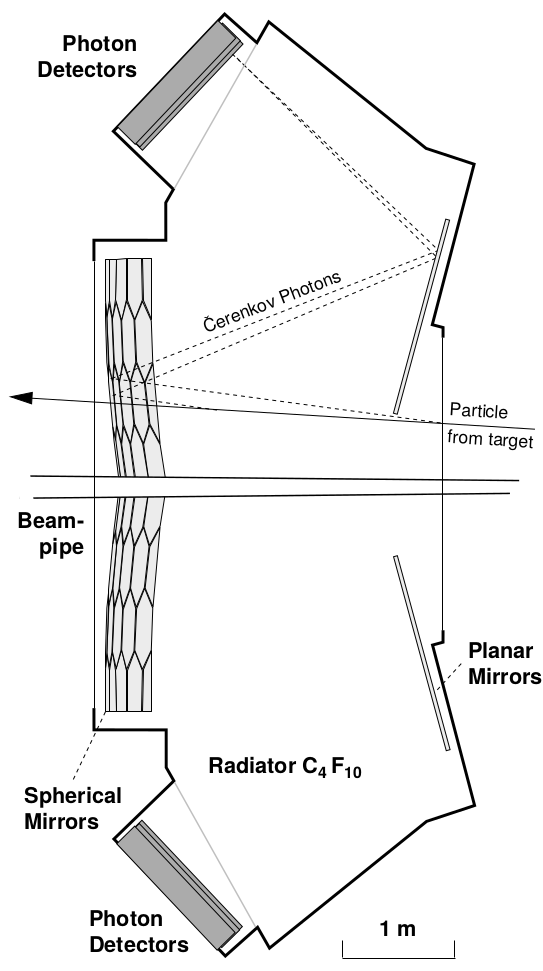
\includegraphics[width=0.9\textwidth]{pictures/HERAb_RICH.png}
\caption{Схема детектора HERA-b RICH.}
\label{fig:HERAbRICH}
\end{minipage}
\hspace{0.01\textwidth}
\begin{minipage}[b]{0.545\textwidth}
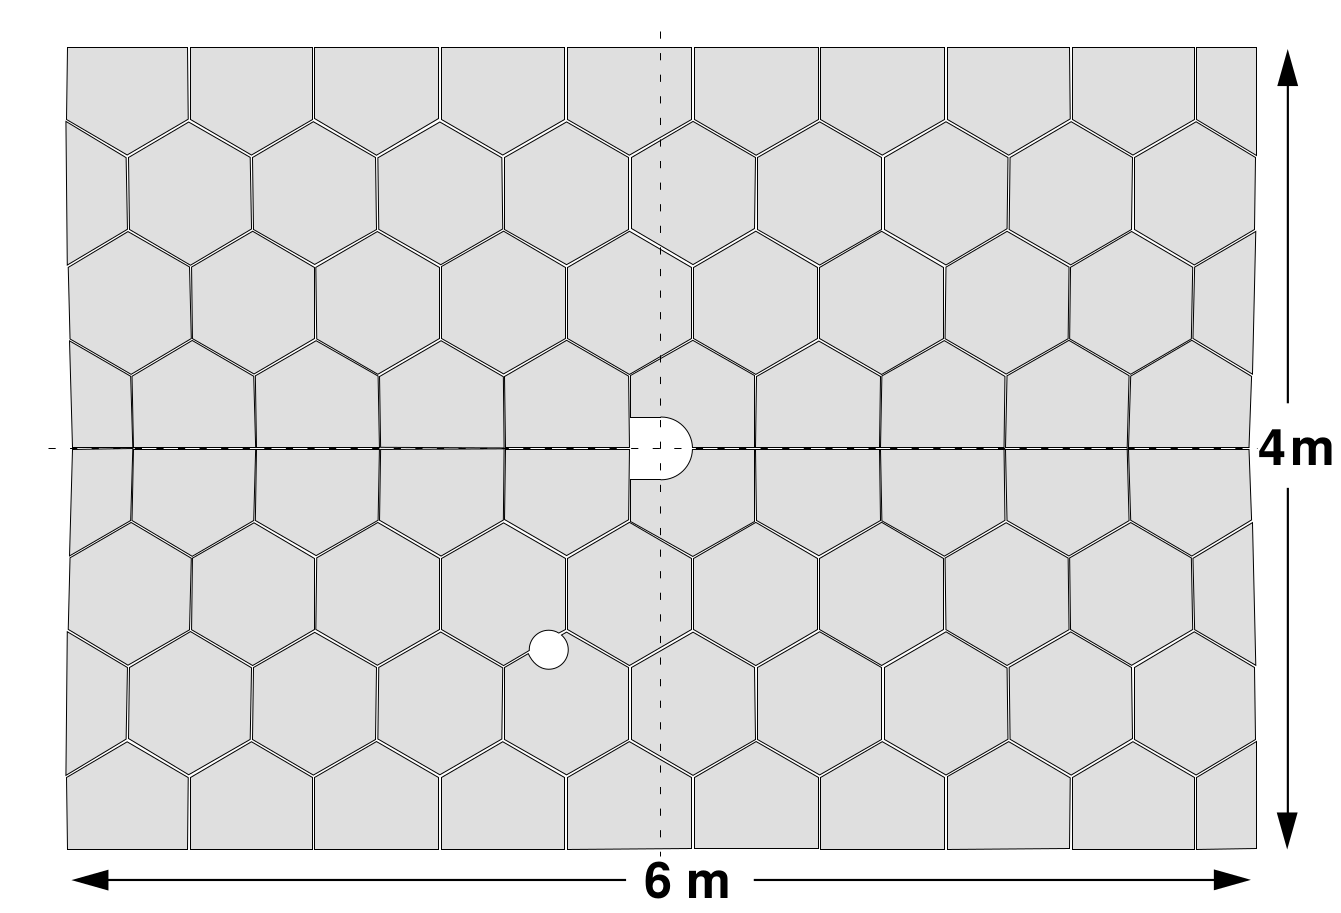
\includegraphics[width=1.0\textwidth]{pictures/HERAb_RICH_mirrors.png}
\caption{Схема компоновки сферических зеркал HERA-b RICH.}
\label{fig:HERAbRICHmirrors}
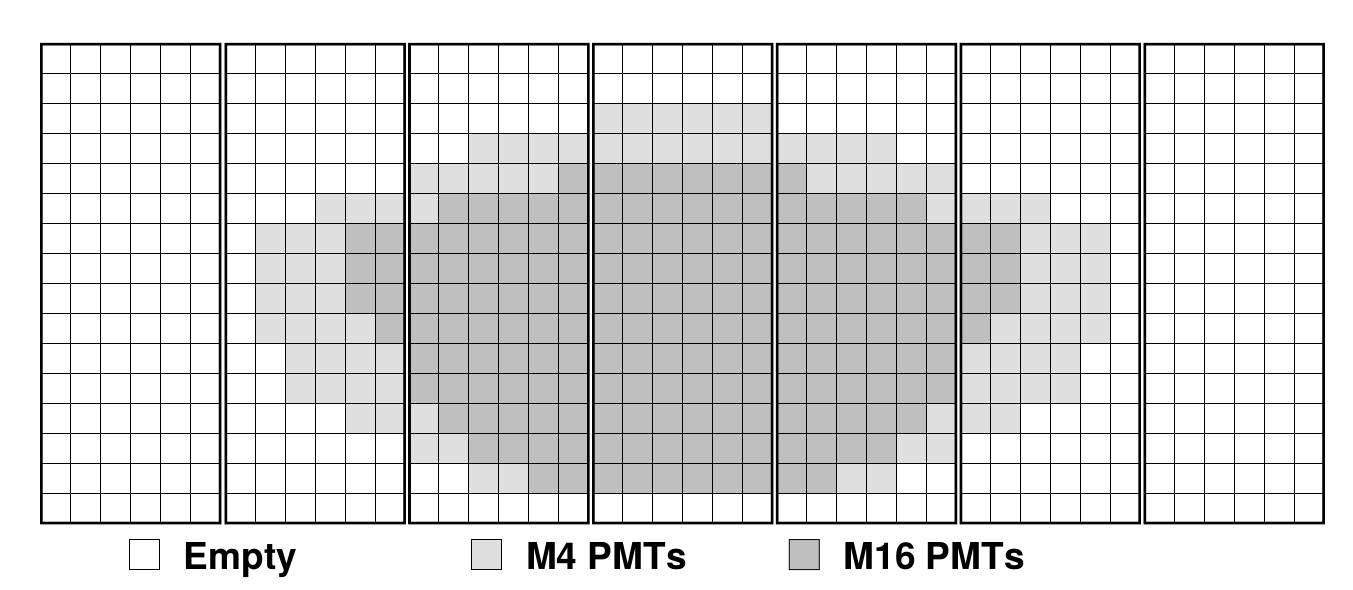
\includegraphics[width=1.0\textwidth]{pictures/HERAb_camera.png}
\caption{Схема заполненности одной фоточувствительной камеры HERA-b RICH. Одна ячейка соответствует модулю из 8~МА~ФЭУ.}
\label{fig:HERAbRICHcamera}
\end{minipage}
\end{figure}
